\FloatBarrier
\begin{figure}[ht!]
    \section{}\label{sec:hardware_images}
    \centering
    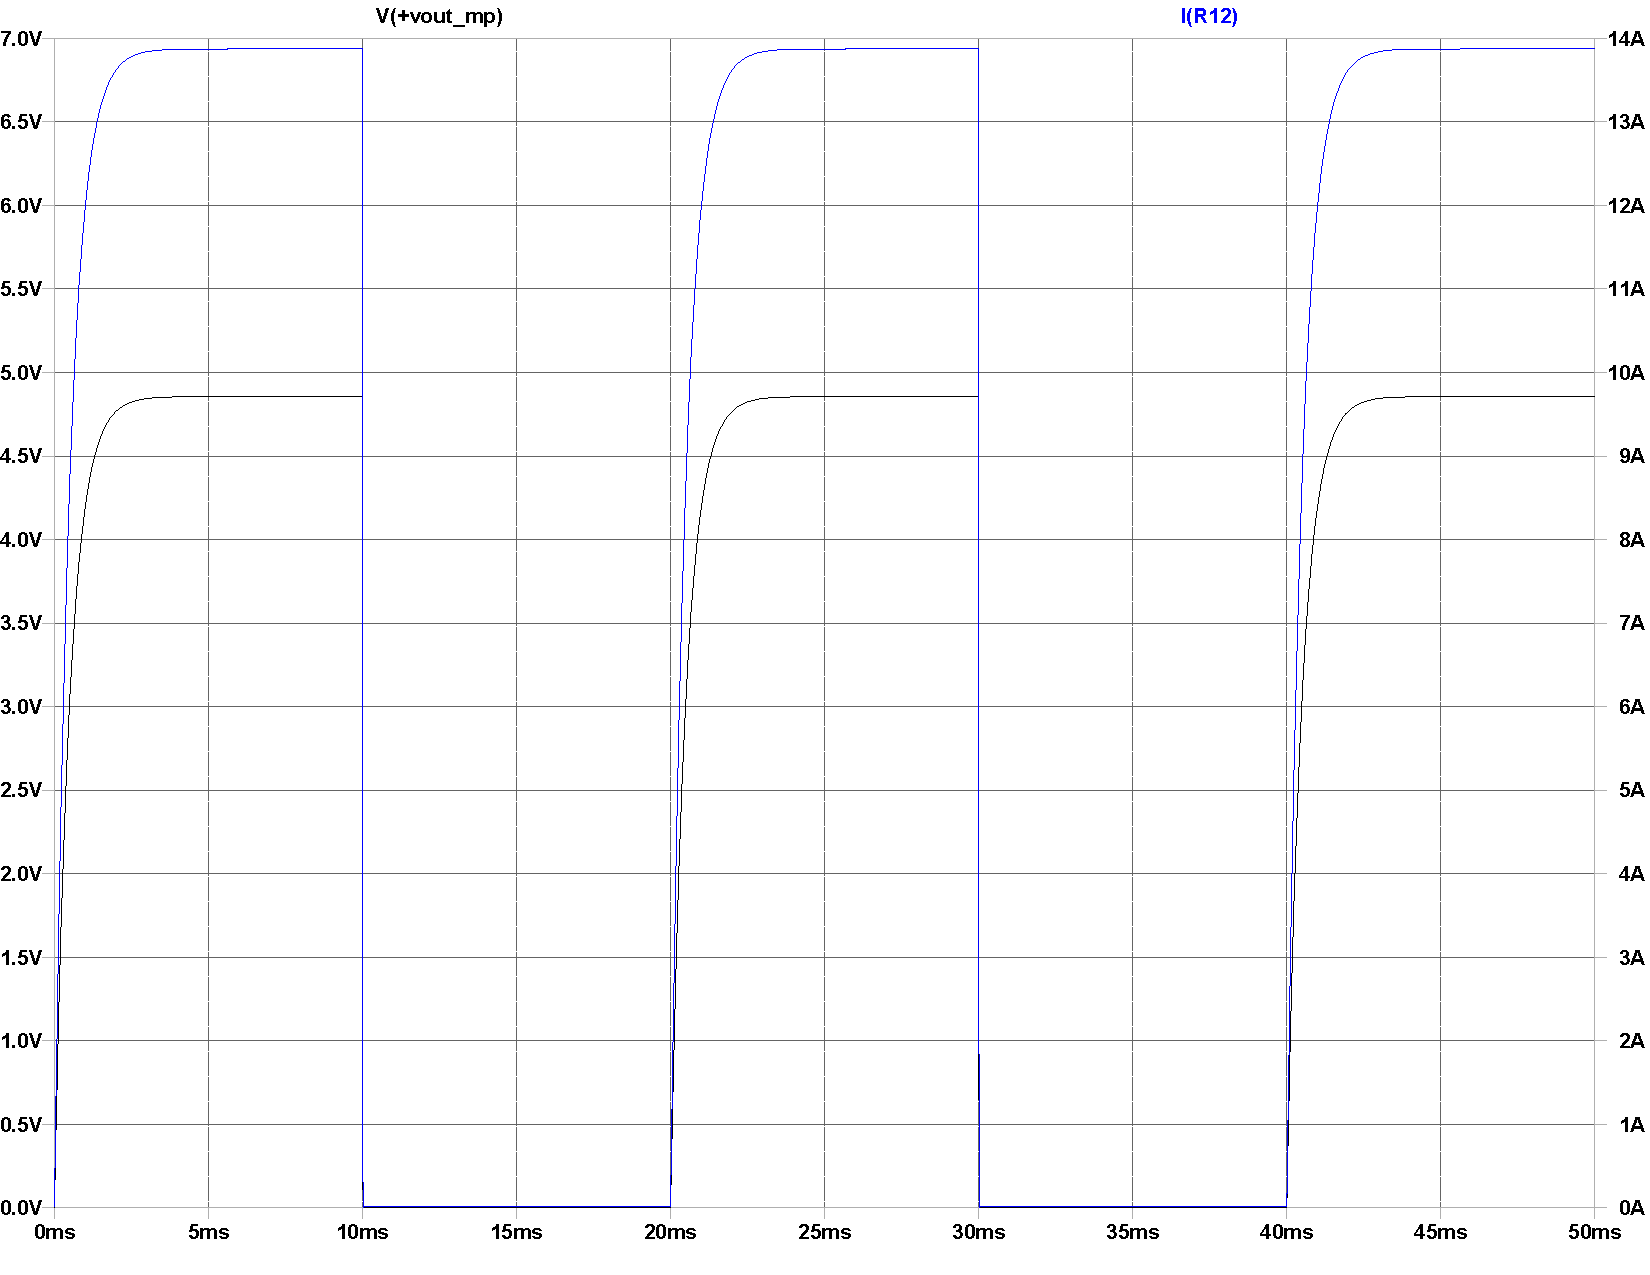
\includegraphics[width=0.45\textwidth]{LT3080-1_Transient-response.pdf}
    \caption{12 A linear regulator transient response.}
    \label{fig:LT3080-1_Transient-response}
\end{figure}

\begin{figure}[ht!]
    \centering
    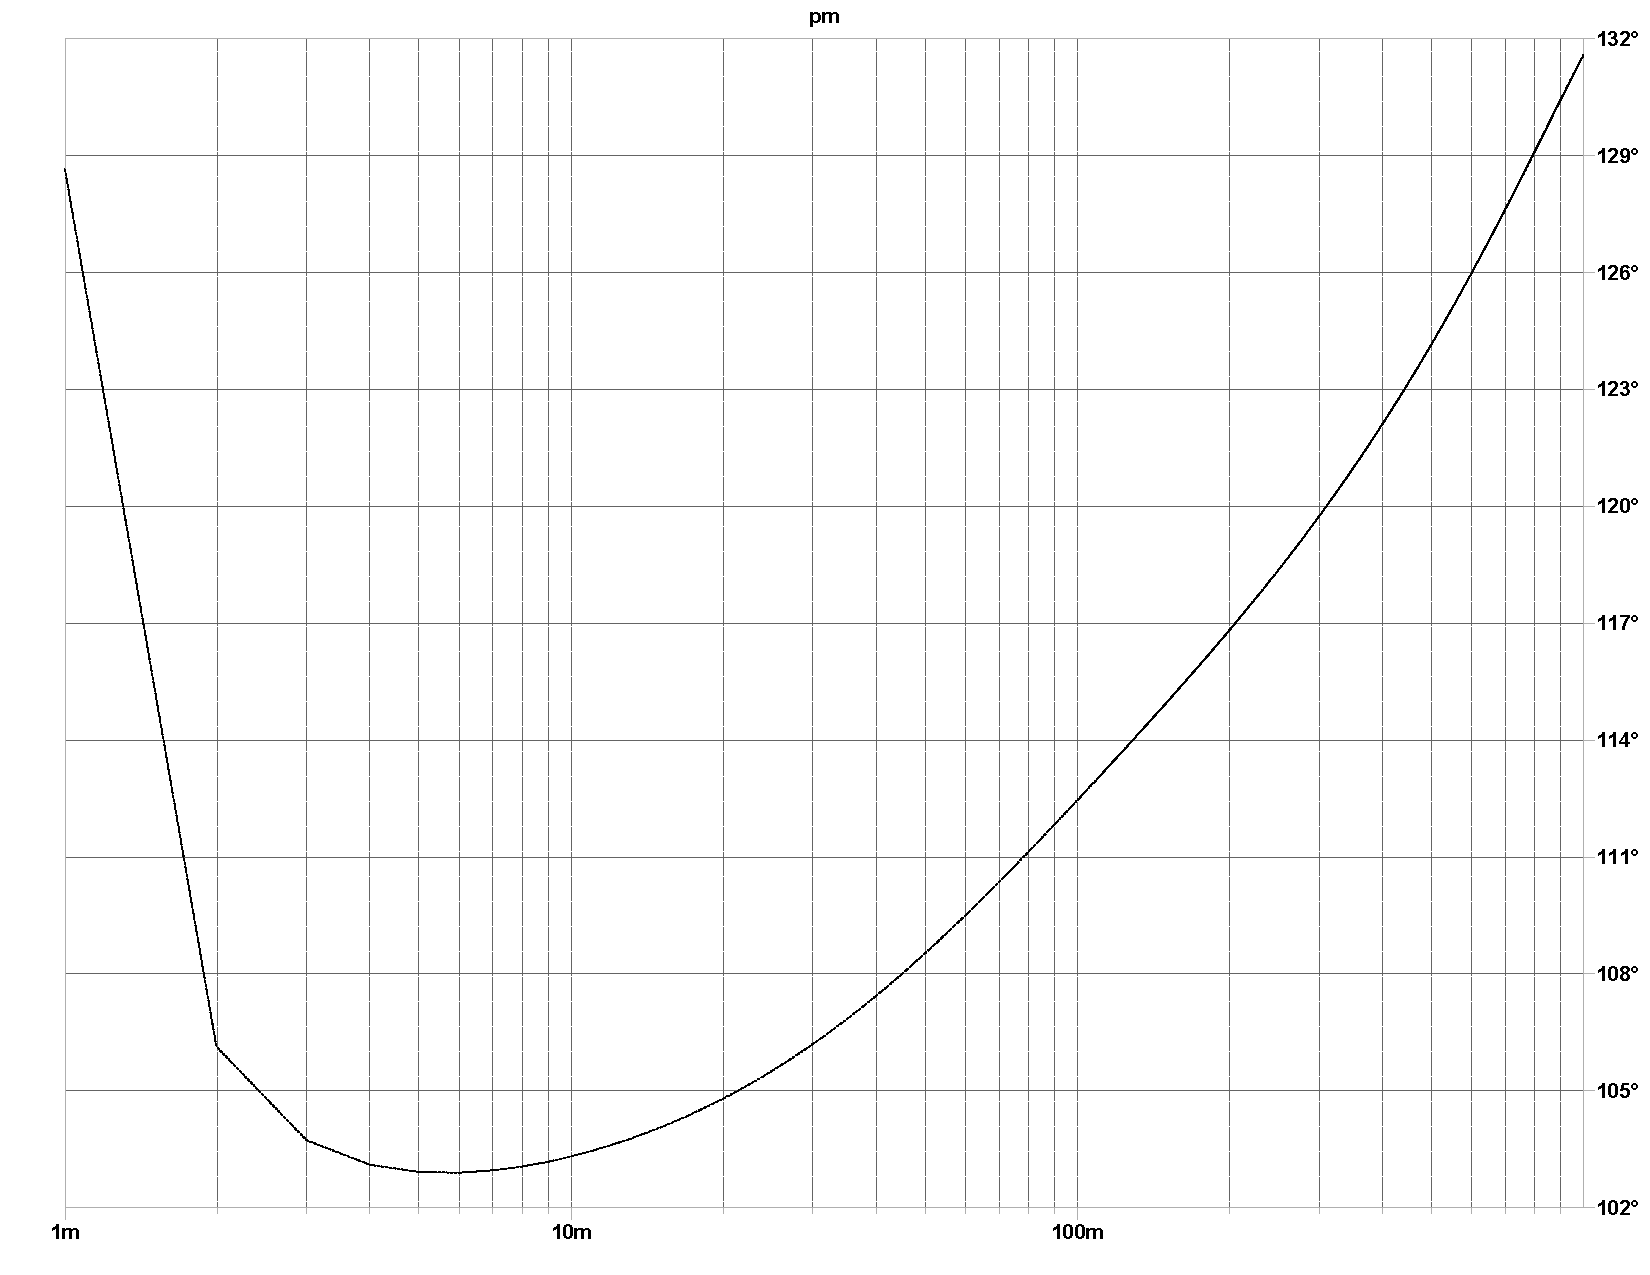
\includegraphics[width=0.45\textwidth]{LT3080-1_Phase-margin_VS_setpoint.pdf}
    \caption{12 A linear regulator phase margin vs set point (current). The gain margin is infinite}
    \label{fig:LT3080-1_Phase-margin_VS_setpoint}
\end{figure}

\begin{figure}[ht!]
    \centering
    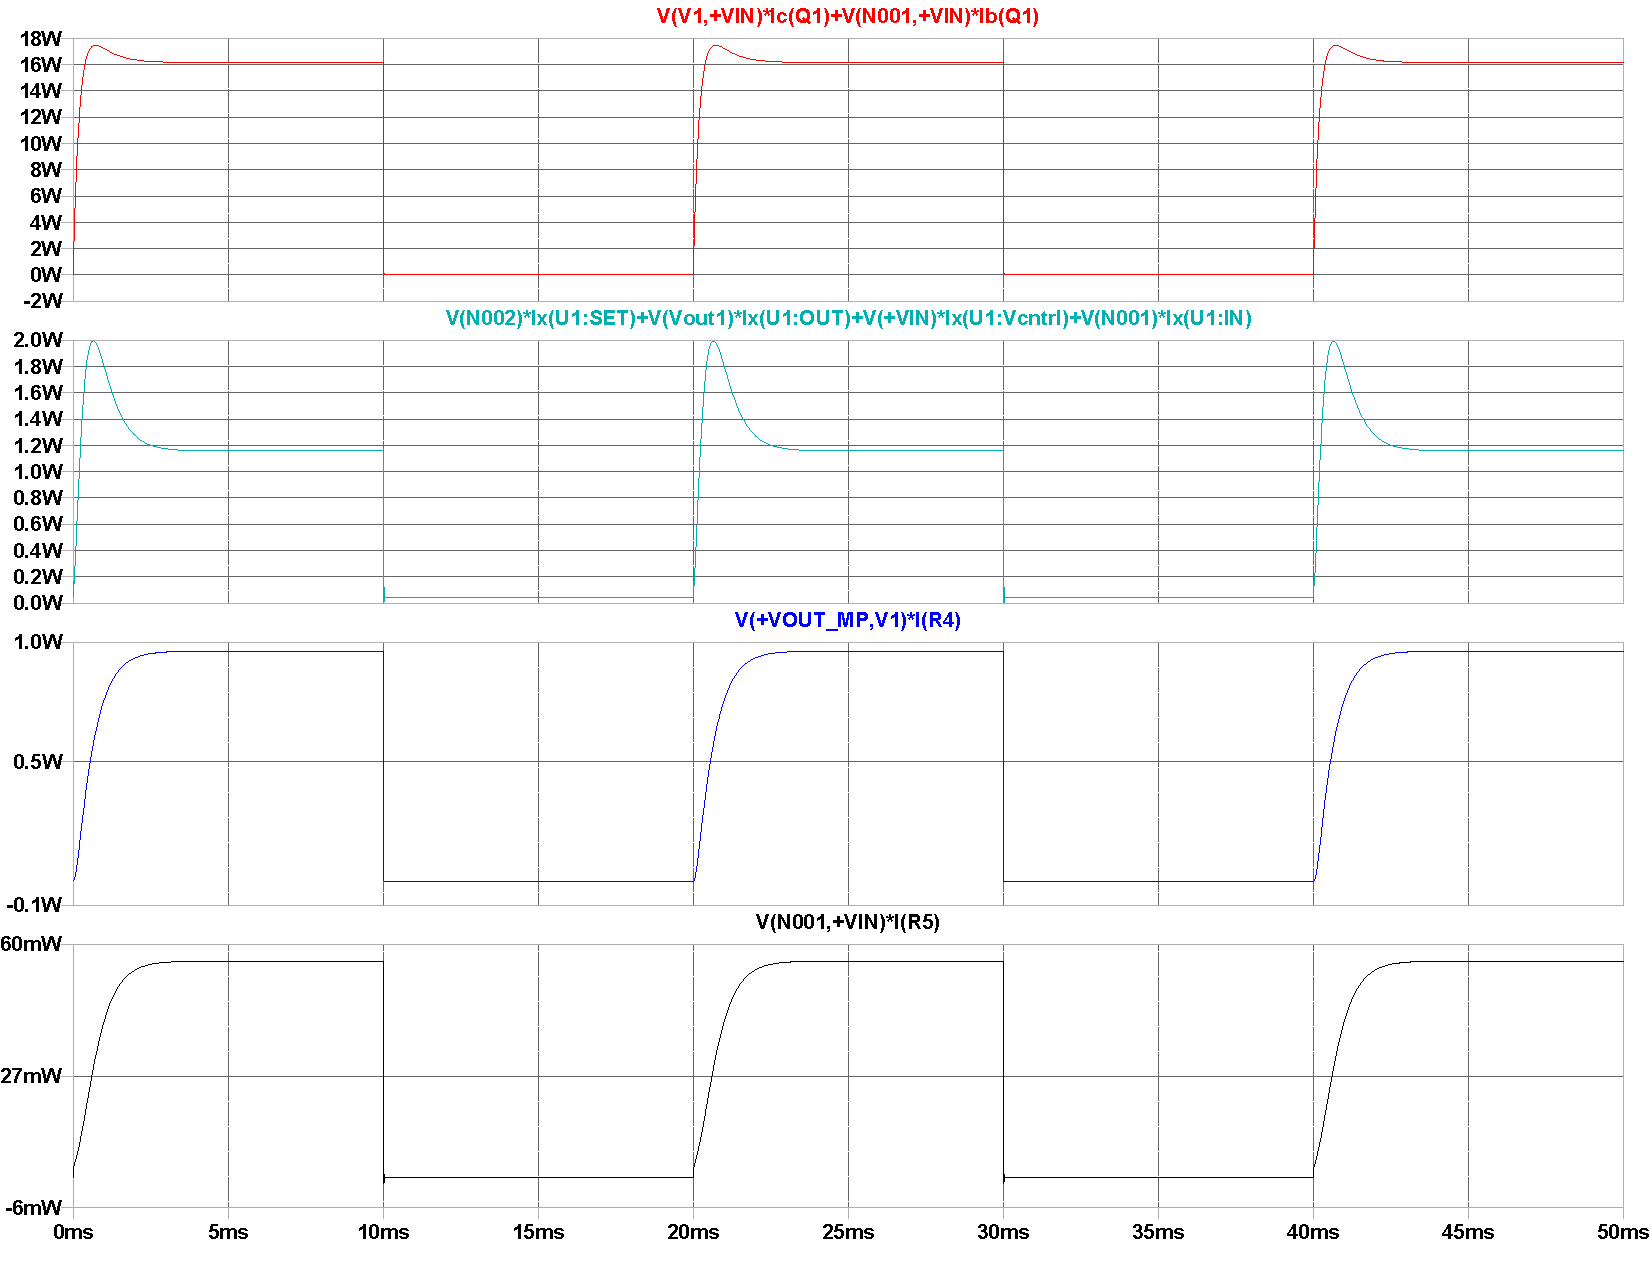
\includegraphics[width=0.45\textwidth]{LT3080-1_PowerDissipation.pdf}
    \caption{12 A linear regulator power dissipation.}
    \label{fig:LT3080-1_PowerDissipation}
\end{figure}

\begin{figure}[ht!]
    \centering
    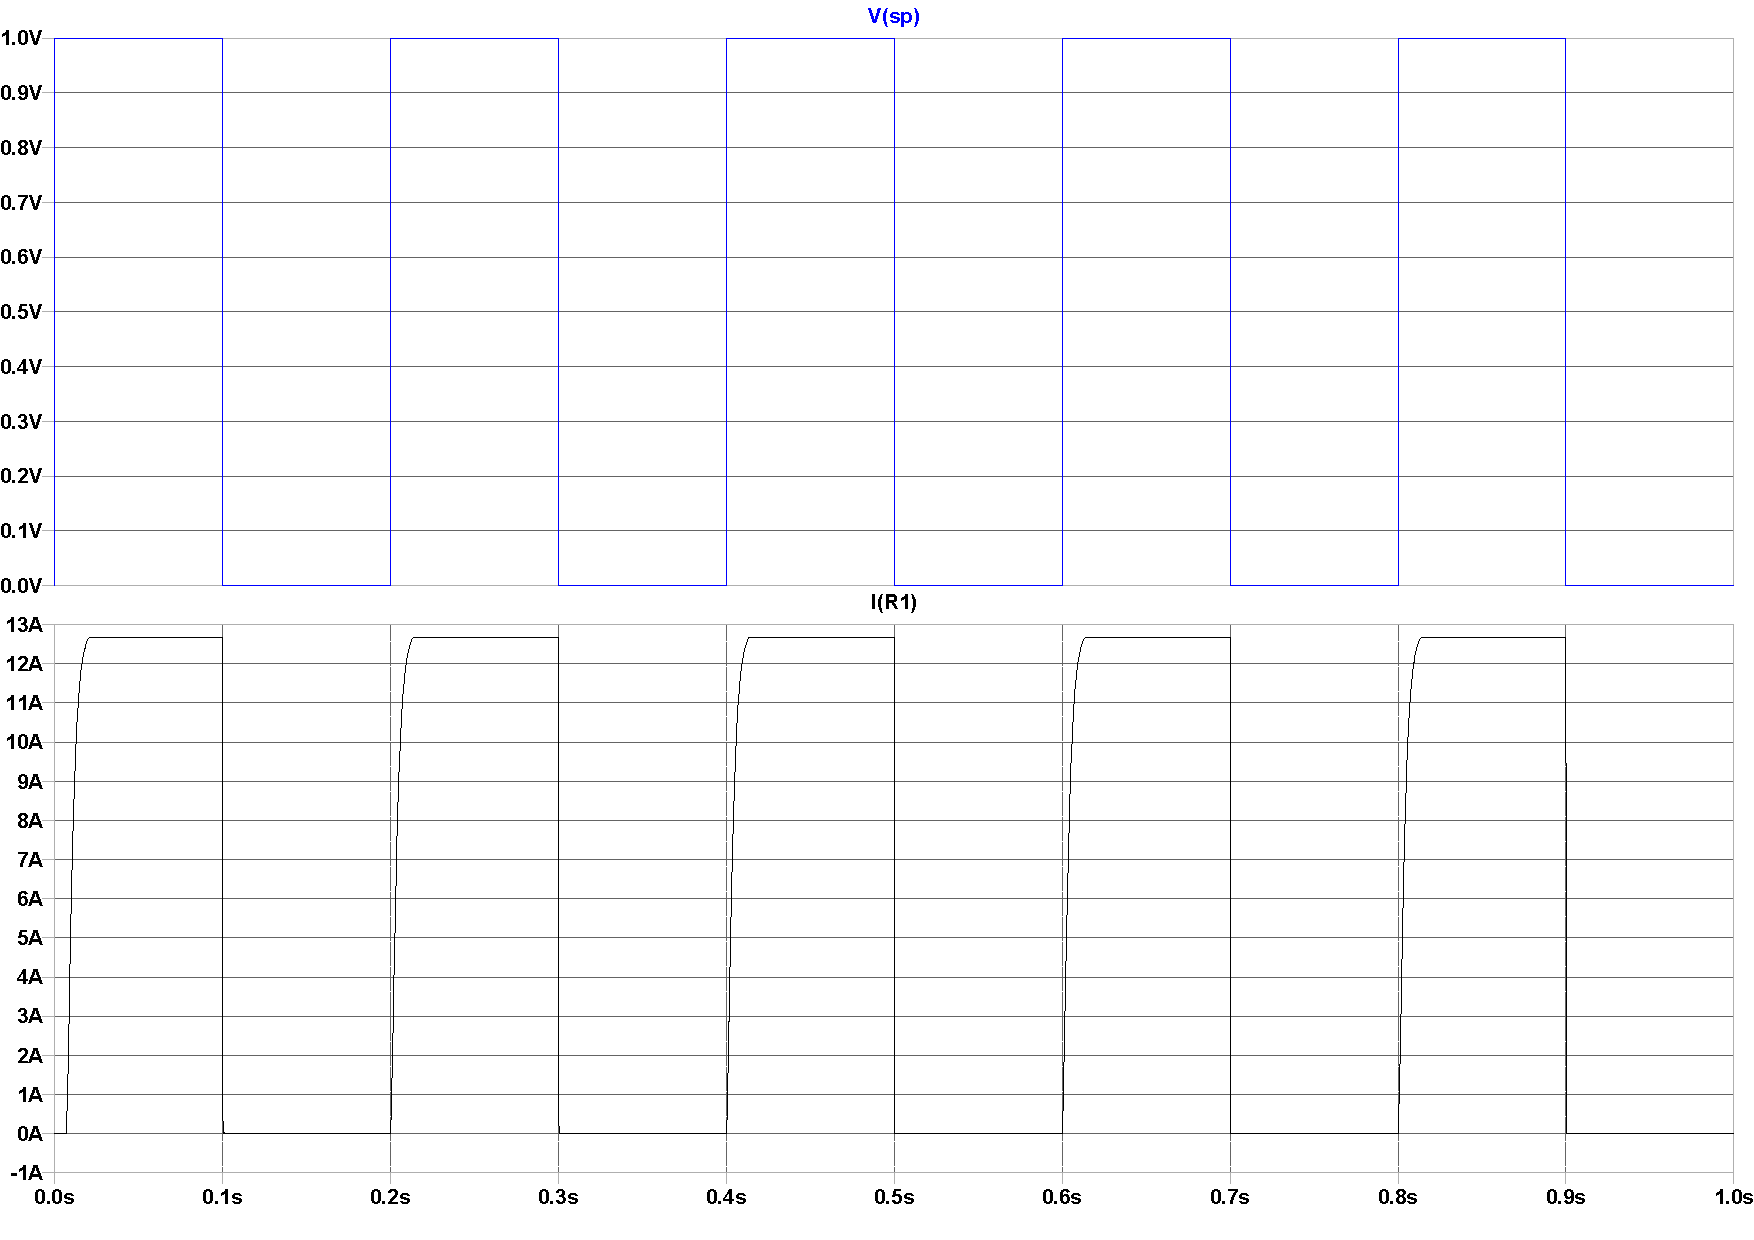
\includegraphics[width=0.45\textwidth]{CurrentSinkTransient.pdf}
    \caption{12 A current sink transient response.}
    \label{fig:CurrentSinkTransient}
\end{figure}

\begin{figure}[ht!]
    \centering
    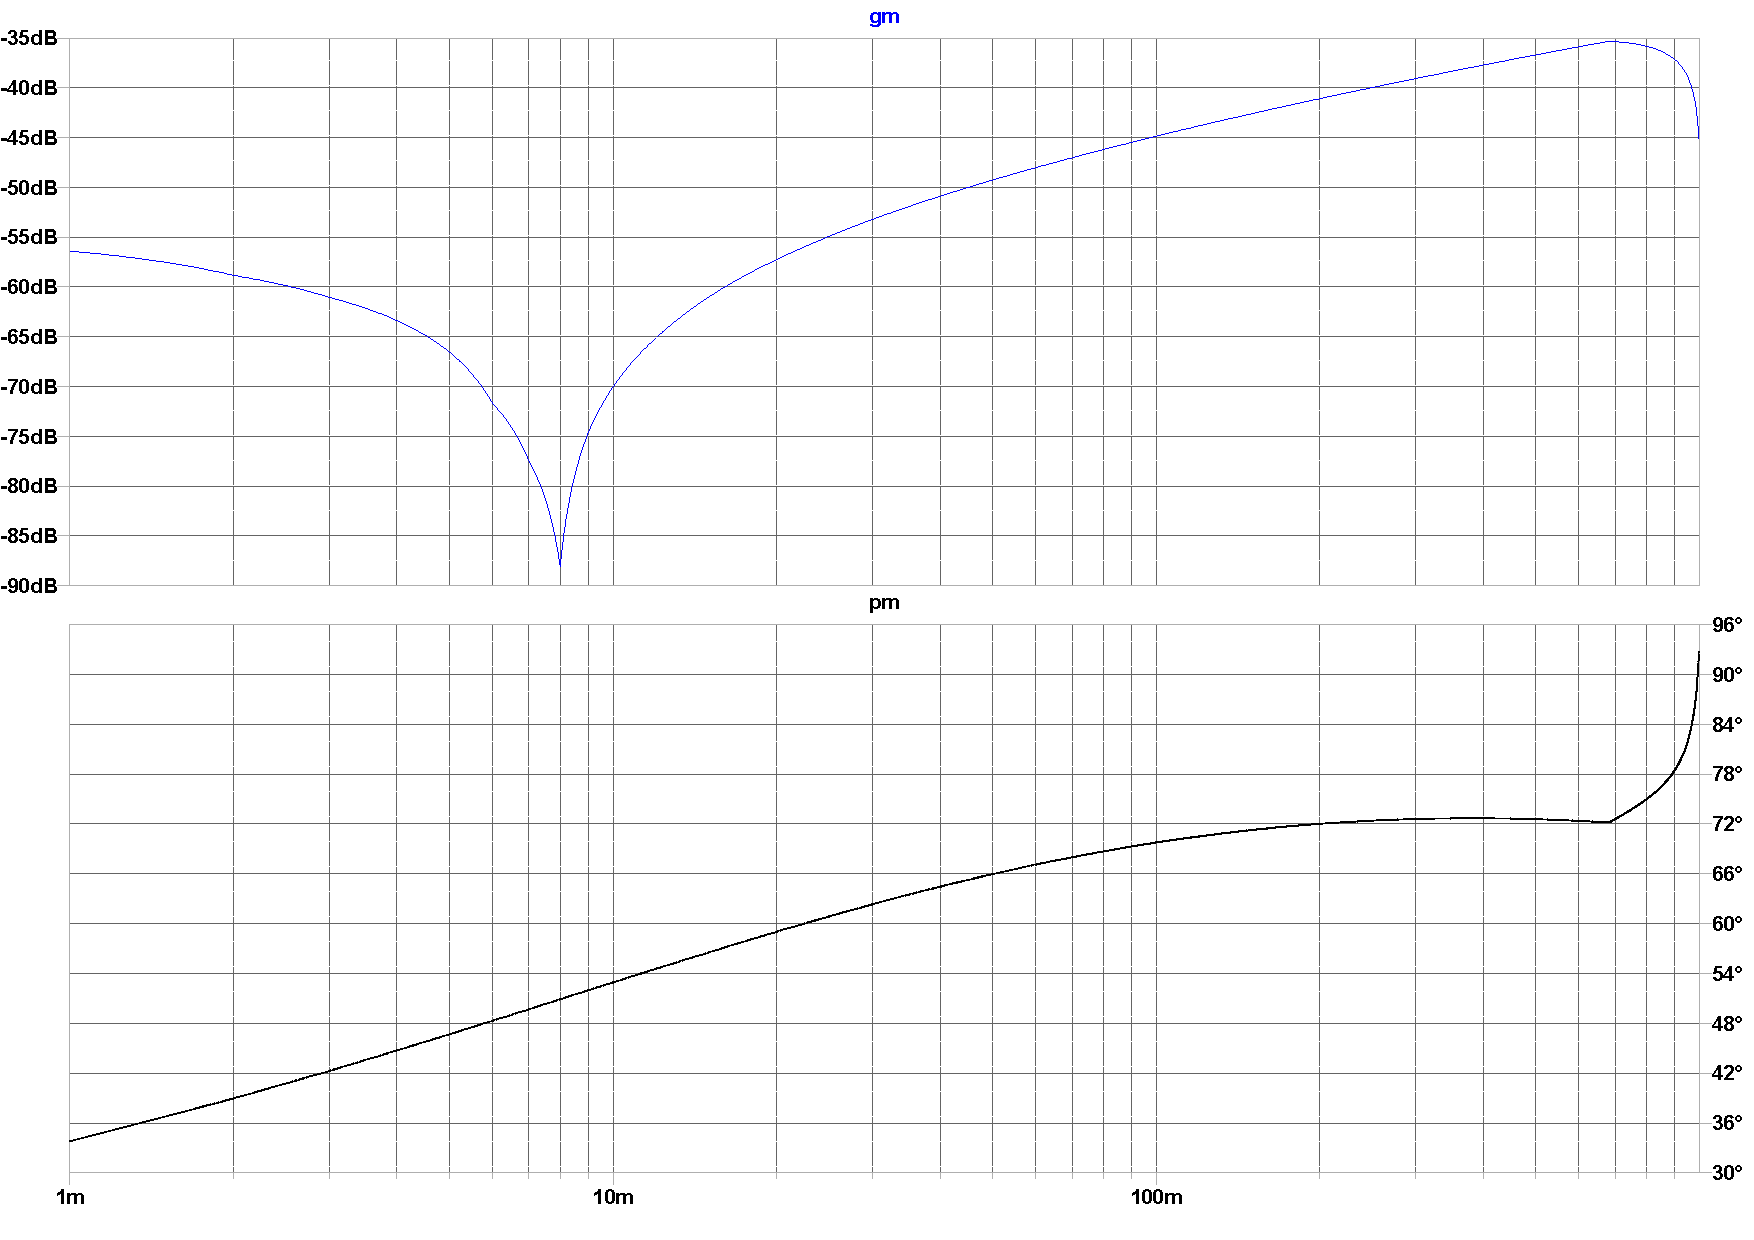
\includegraphics[width=0.45\textwidth]{CurrentSinkPM&GM.pdf}
    \caption{12 A current sink gain (blue) and fase (black) margin.}
    \label{fig:CurrentSinkPM&GM}
\end{figure}

\begin{figure}[ht!]
    \centering
    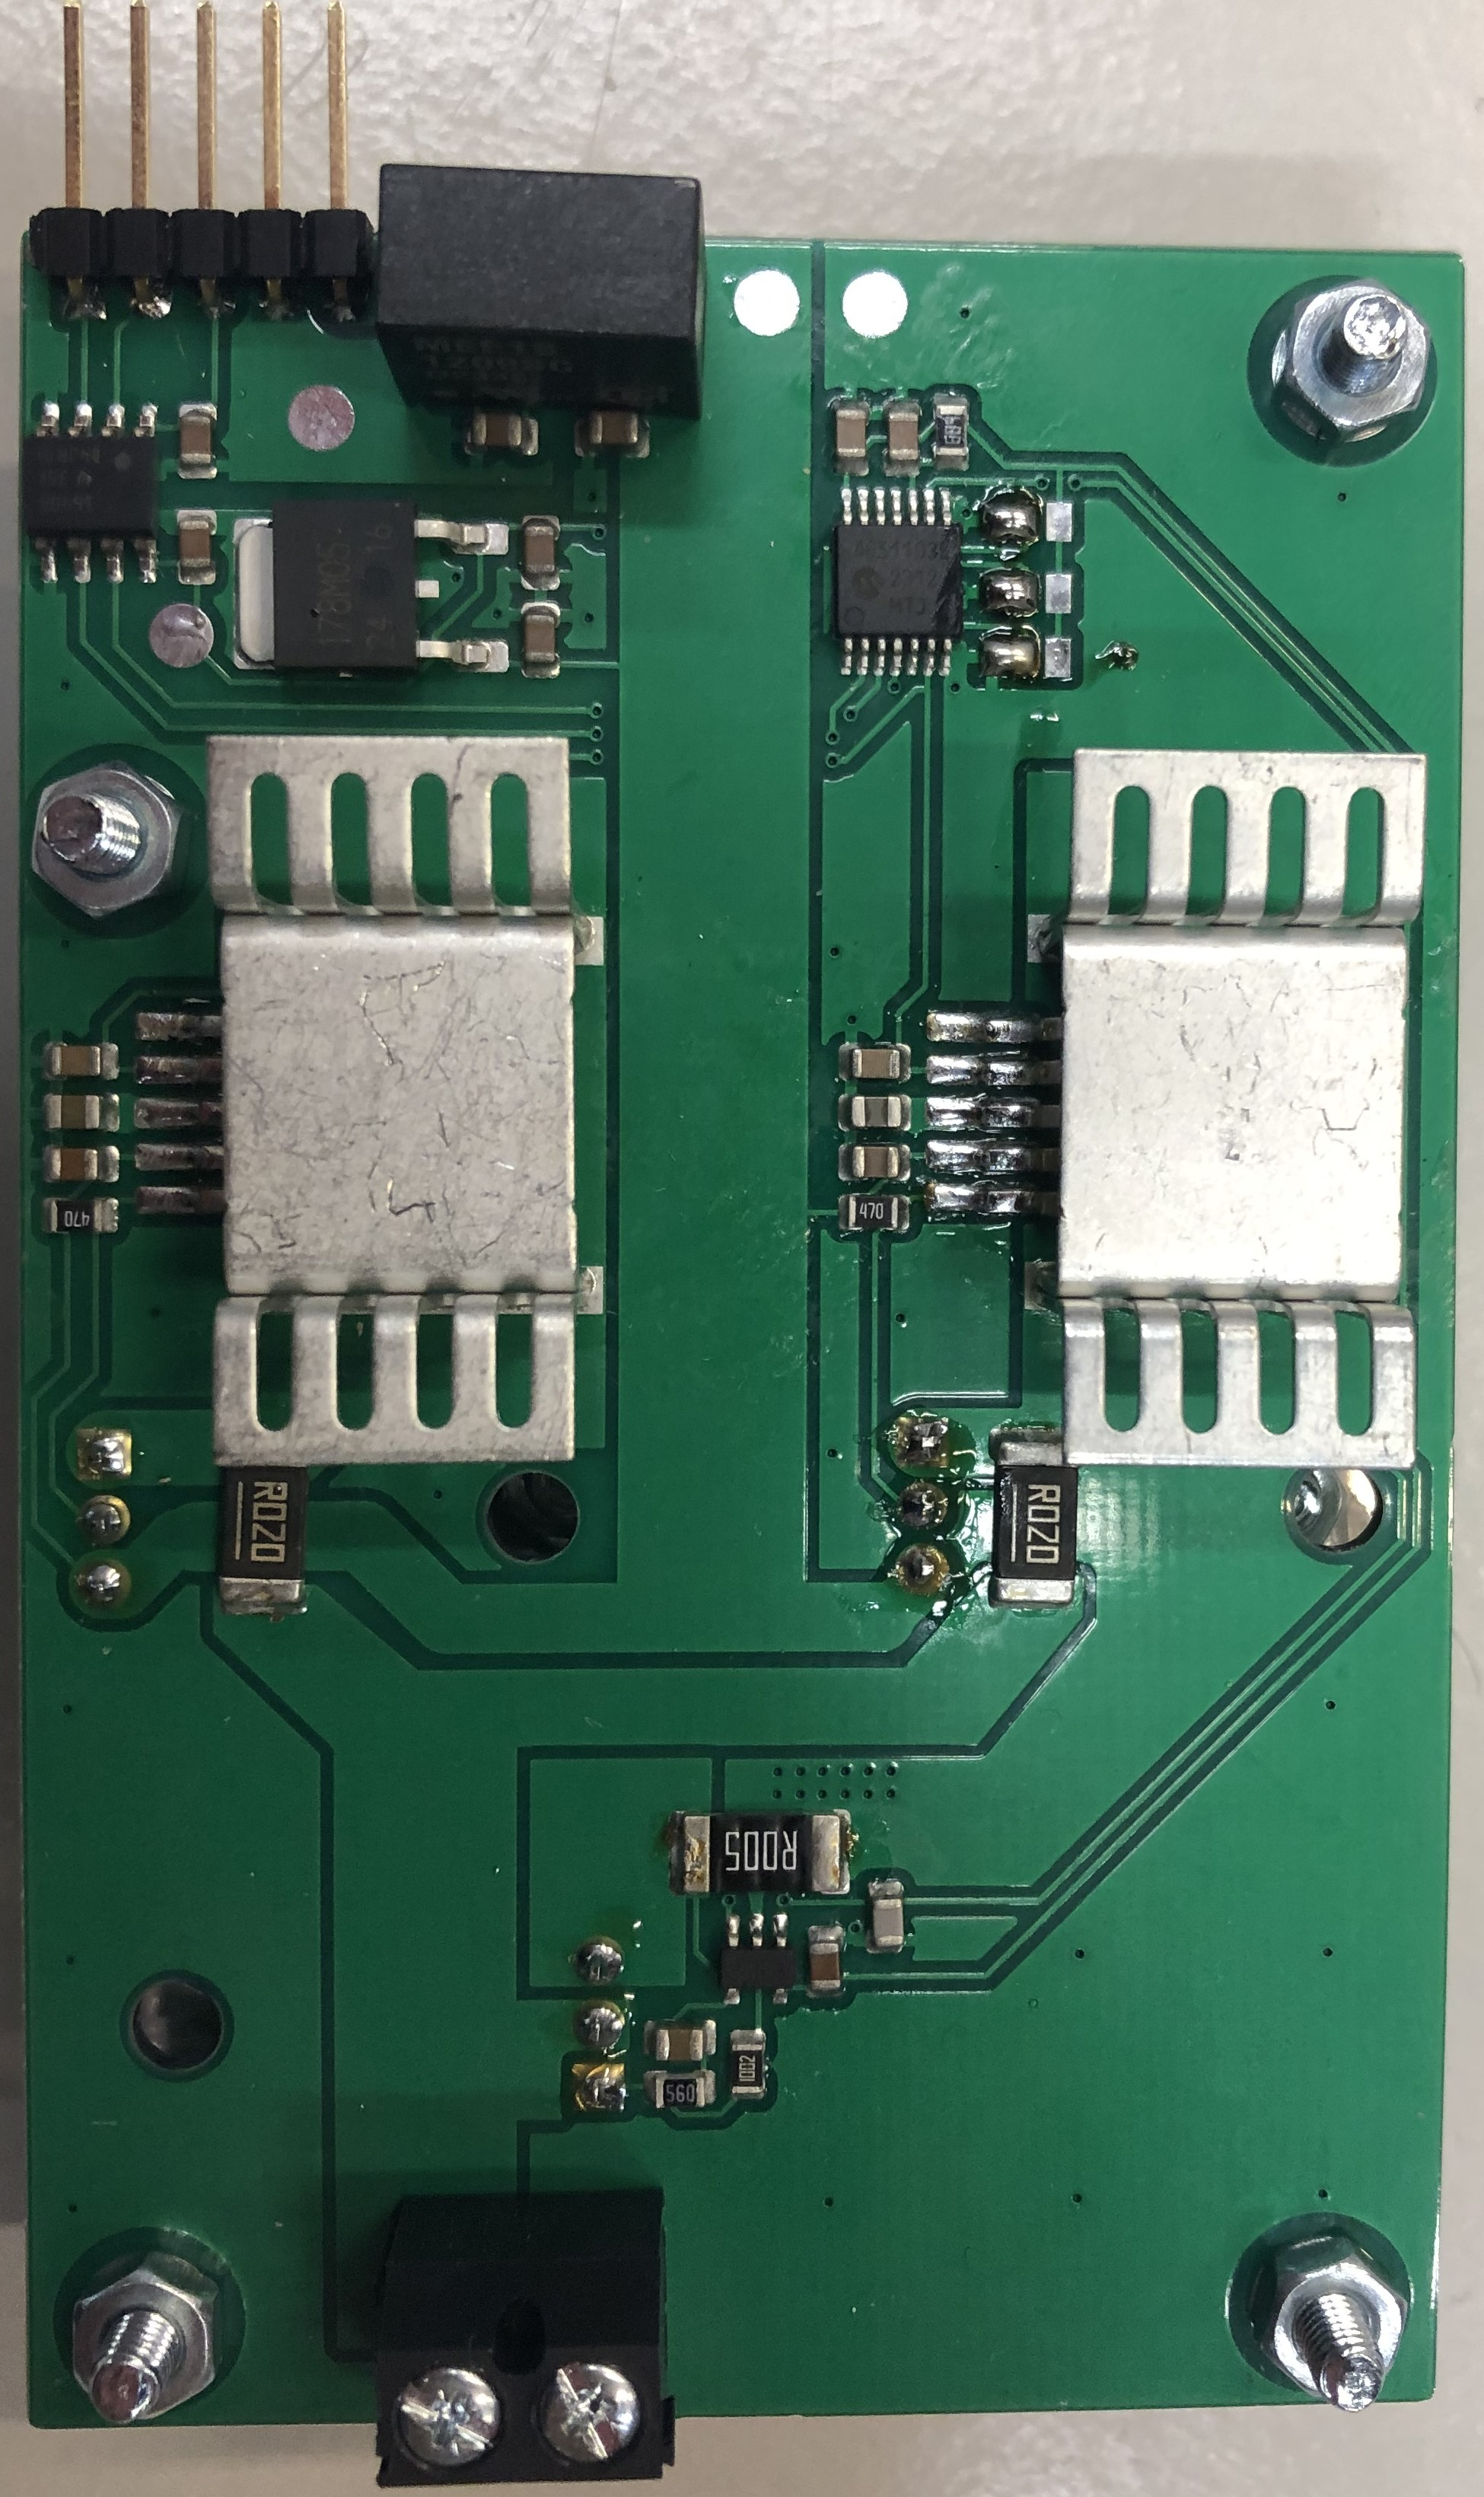
\includegraphics[width=0.45\textwidth]{CellBoardTop.jpg}
    \caption{Top view of cell board.}
    \label{fig:CellBoardTop}
\end{figure}

\begin{figure}[ht!]
    \centering
    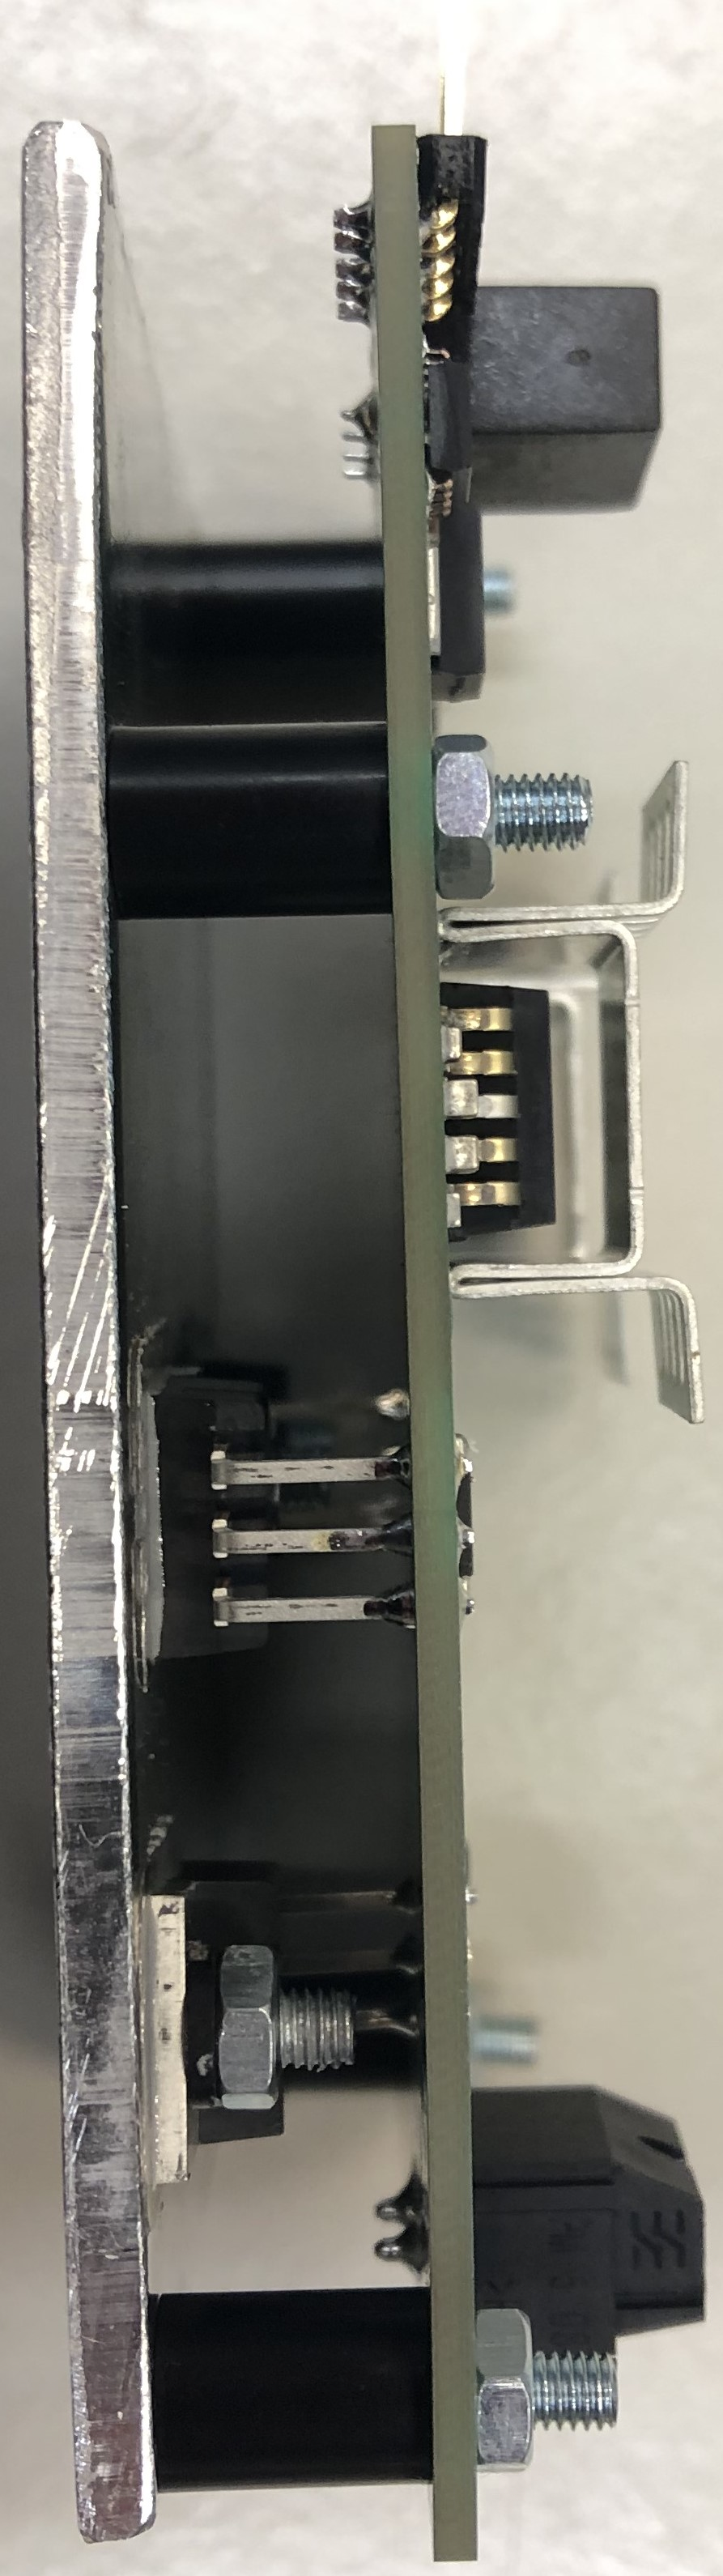
\includegraphics[height=0.45\textwidth,angle=90,origin=c]{CellBoardSide.jpg}
    \caption{Side view of cell board.}
    \label{fig:CellBoardSide}
\end{figure}

\begin{figure}[ht!]
    \centering
    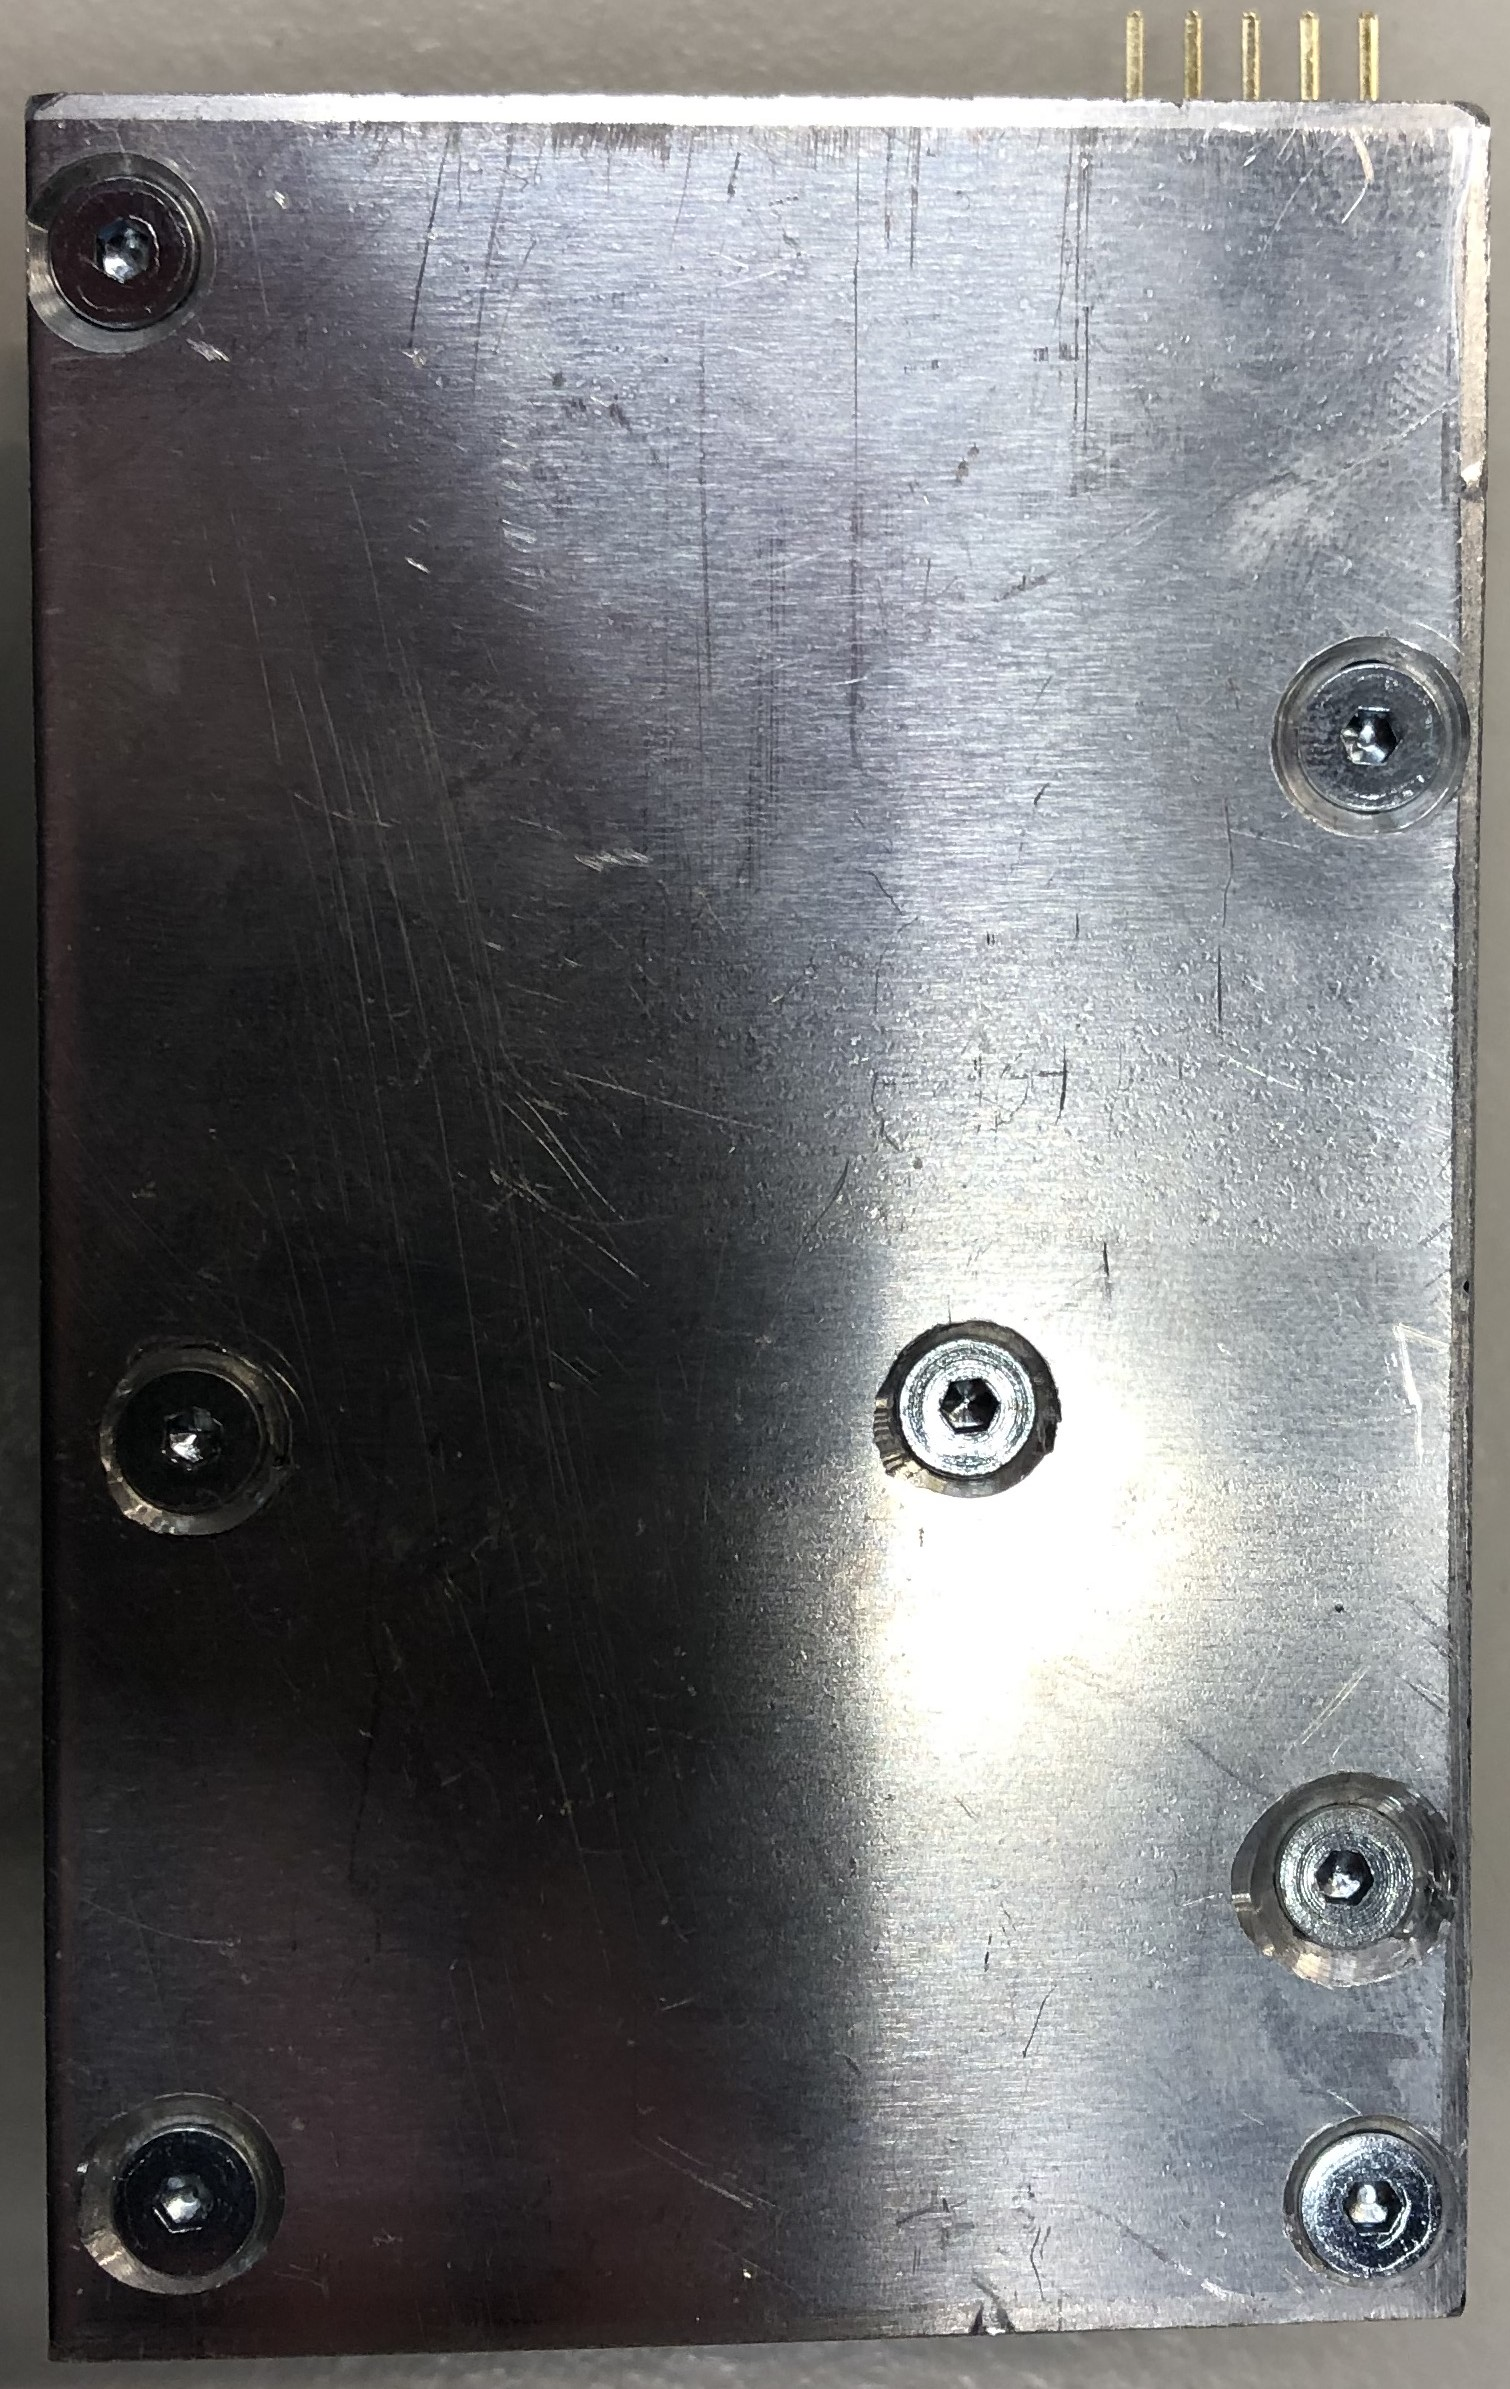
\includegraphics[width=0.45\textwidth]{CellBoardBottom.jpg}
    \caption{Bottom view of cell board.}
    \label{fig:CellBoardBottom}
\end{figure}

\begin{figure}[ht!]
    \centering
    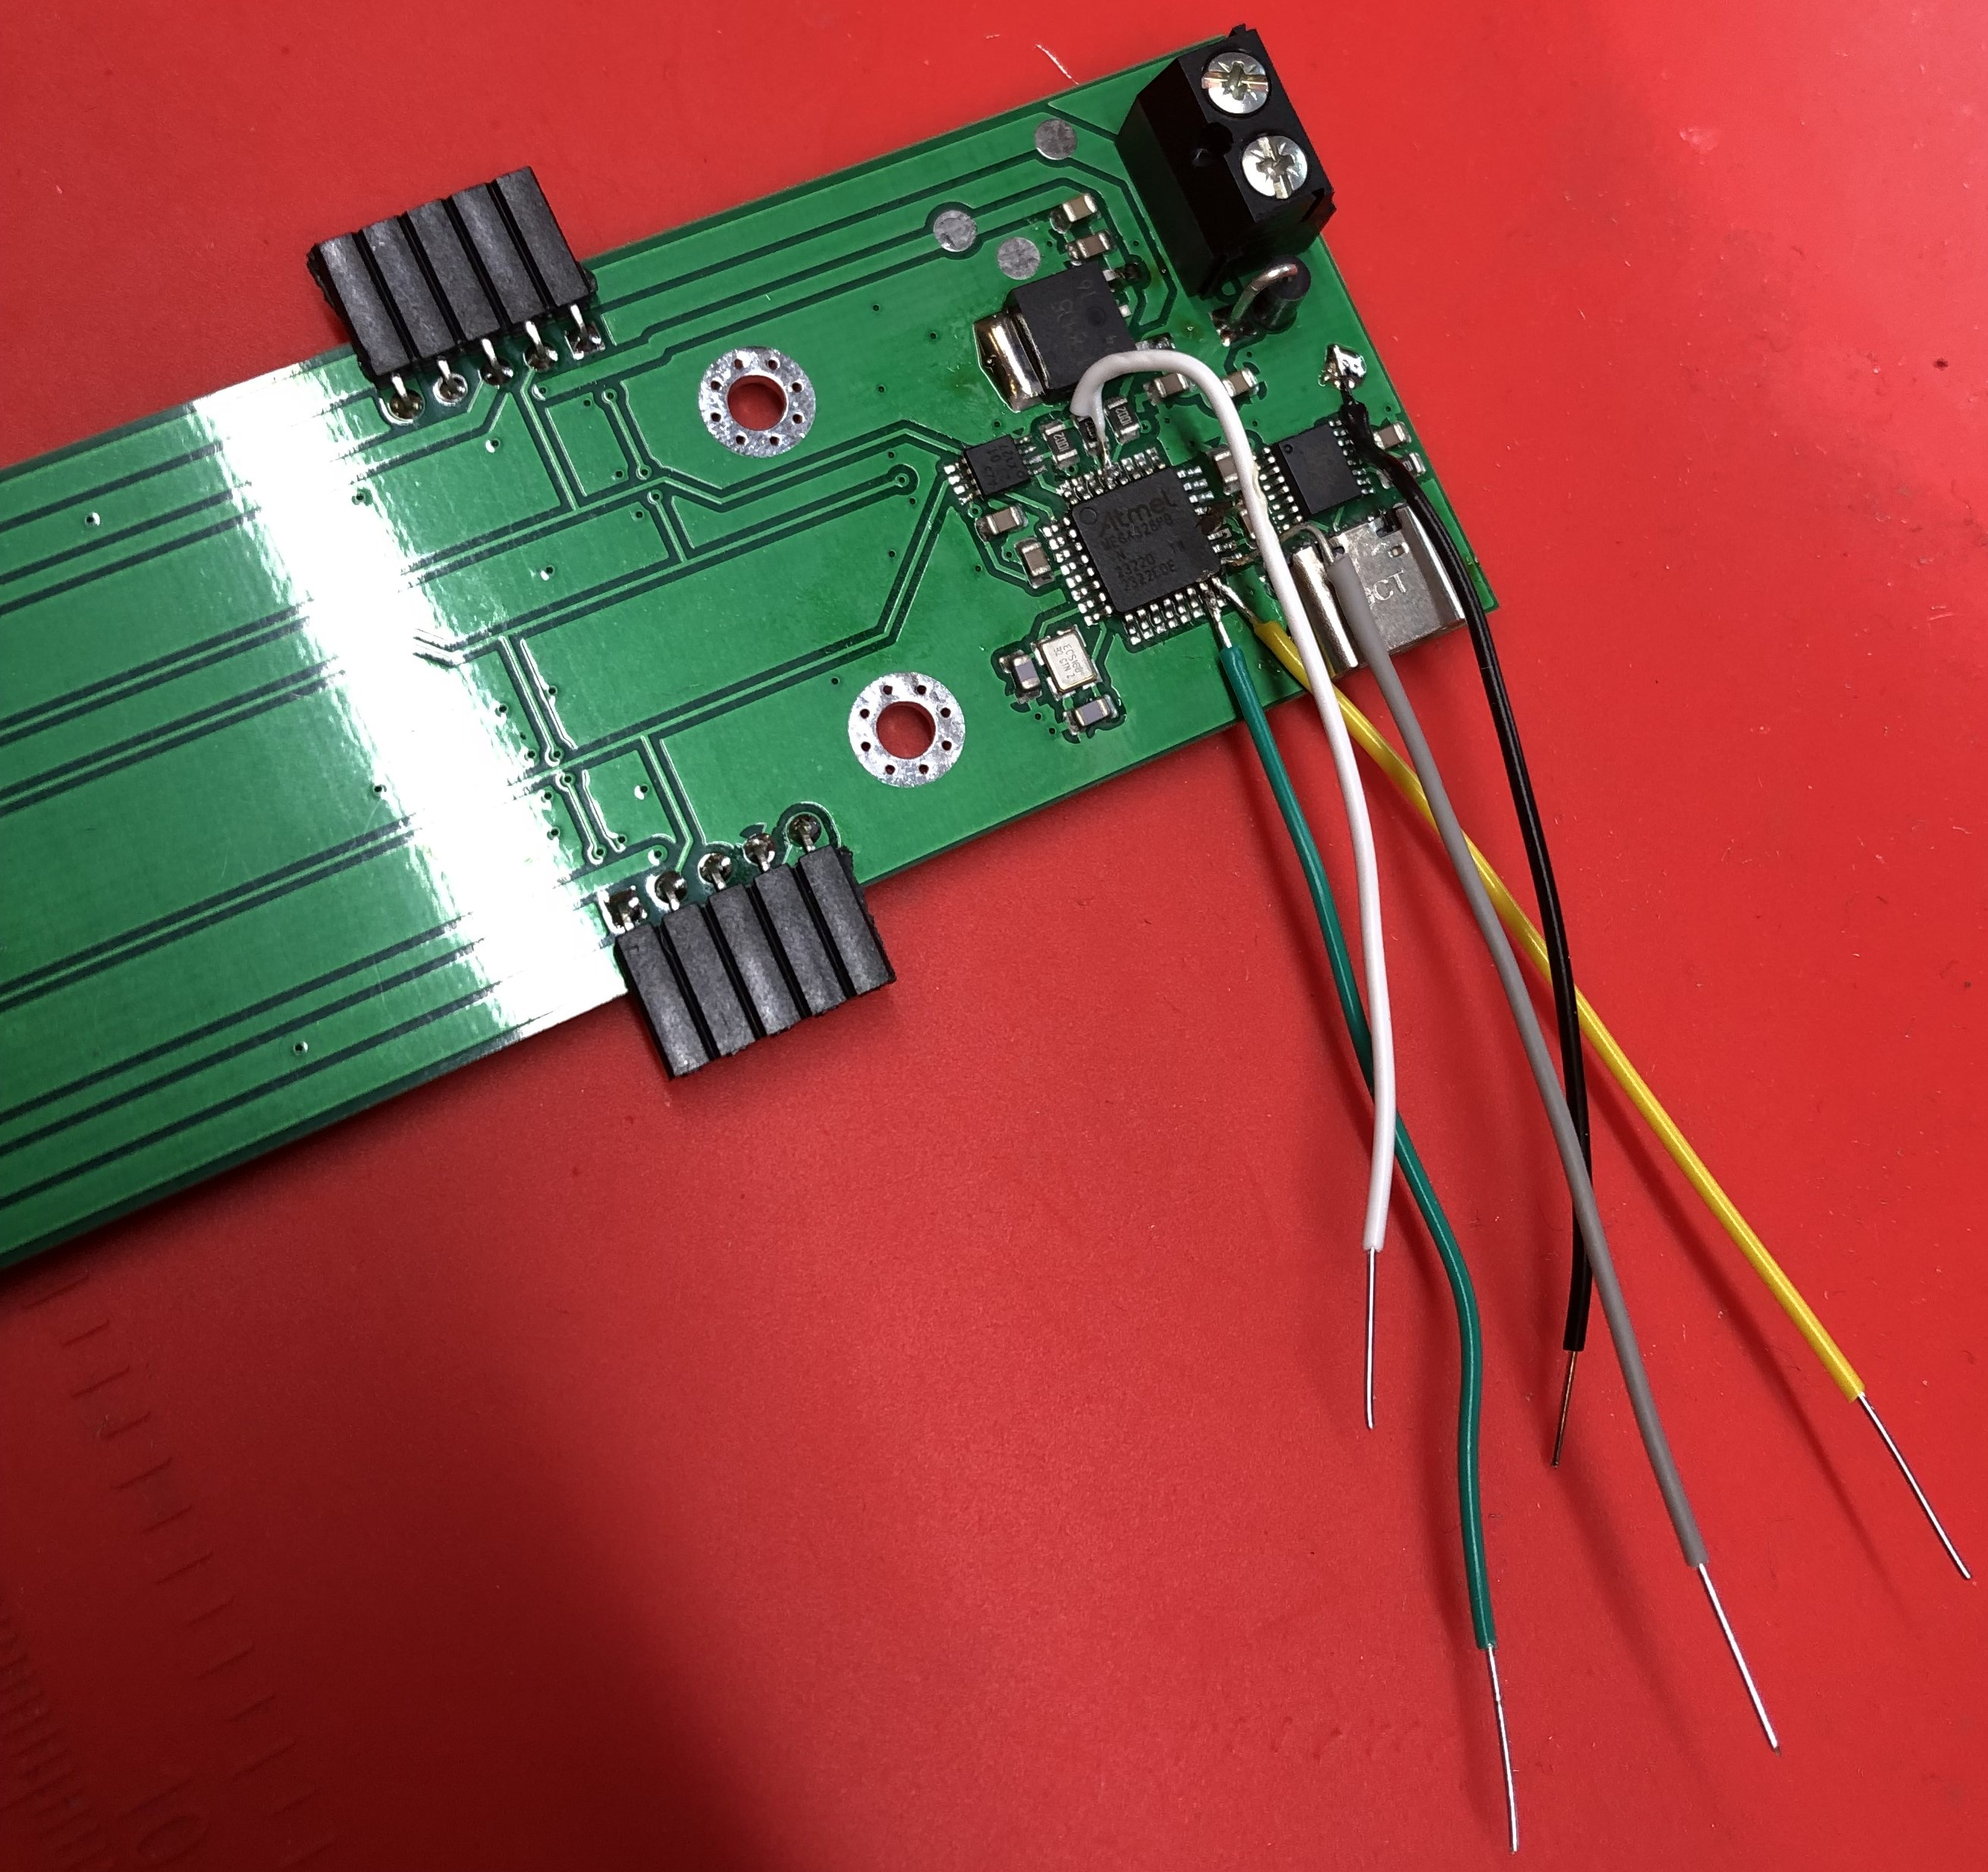
\includegraphics[height=0.95\textheight]{ModelBoardTop.jpg}
    \caption{Top view of model board.}
    \label{fig:ModelBoardTop}
\end{figure}

\begin{figure}[h!]
    \centering
    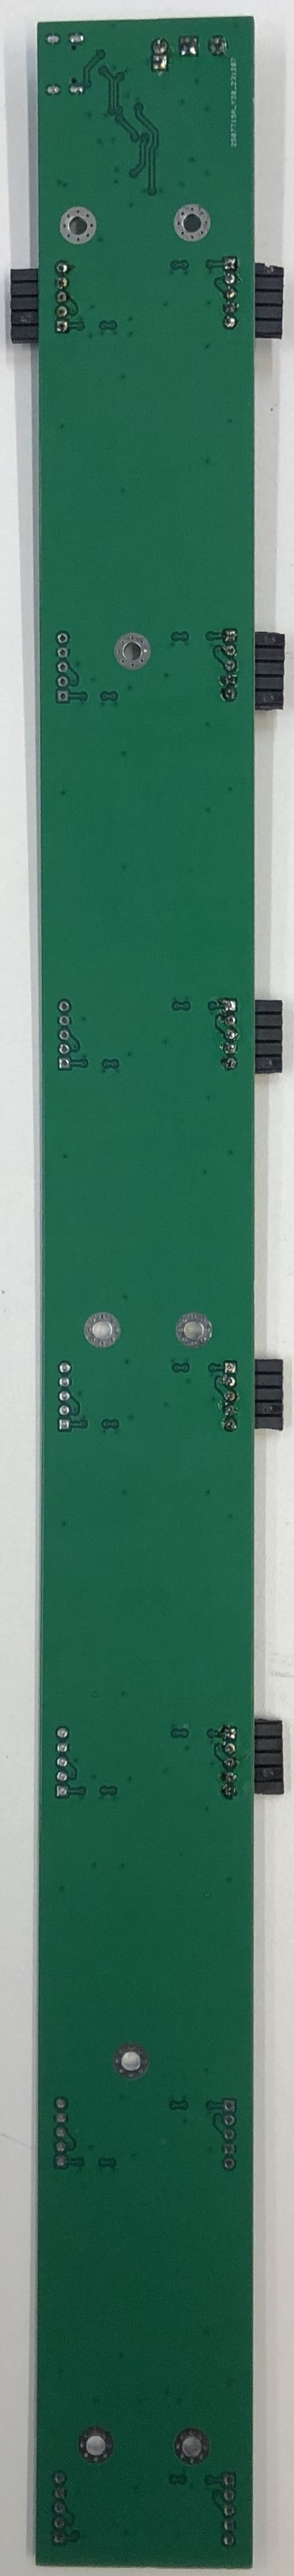
\includegraphics[height=0.95\textheight]{ModelBoardBottom.jpg}
    \caption{Bottom view of model board.}
    \label{fig:ModelBoardBottom}
\end{figure}
\FloatBarrier